\documentclass[11pt,a4paper]{article}
\usepackage[utf8x]{inputenc}
\usepackage[T1]{fontenc}
%\usepackage{gentium}
\usepackage{mathptmx} % Use Times Font

\usepackage{graphicx} % Required for including pictures
\usepackage{hyperref} % Format links for pdf
\usepackage[british]{babel} % Multilingual bibliographies
\usepackage{natbib}
\setlength{\bibsep}{0.0pt}

\frenchspacing % No double spacing between sentences
\usepackage[margin=1in]{geometry}

\usepackage[all]{nowidow} % Tries to remove widows
\usepackage[protrusion=true,expansion=true]{microtype} % Improves typography, load after fontpackage is selected

\usepackage{lipsum} % Used for inserting dummy 'Lorem ipsum' text into the template

\title{Degree variability and grade inflation in UK higher education}
\author{Zihao Cai, Litu Ou and Ki Zhou}
%\usepackage{natbib}

\begin{document}

\maketitle

%% INSTRUCTIONS:
%%
%% 1. Please rename this file fds-project-option-1.tex,
%% fds-project-option-2.tex, or fds-project-option-3.tex, depending on
%% which project option you are doing. When you submit, please submit
%% the PDF file with the corresponding name.
%% 
%% 2. You can edit either using:
%%
%%    a. Overleaf professional, a collabaratorive LaTeX editor. See
%%       https://www.overleaf.com/edu/edinburgh for documentation. Create an
%%       empty document, and copy the files in this directory to it.
%%
%%    b. A LaTeX editor on your PC - you can commit changes to this
%%       repository to collaborate.
%% 
%% 3. Please keep the section and paragraph headings as they are.
%%
%% 4. The word limit for the Overview section is mandatory. For the
%% other sections word limits are suggested.
%%
%% 5. The page limits must be strictkly adhered to, and depend on if
%% you are working individually, in pairs or in threes:
%%
%%   - Individual: 6 pages 
%%   - Pairs: 8 pages 
%%   - Threes: 10 pages 
%%

\section{Overview}
% 250 words maximum

University grading, serving as an evaluation on future generations, has always been an active field of research. This work explores the variability of grades in UK higher education. We visualize the distribution of degrees in different Higher Education Providers, investigate the variation of first-class over time and analyze differences between institutions in different countries of UK, subject studied, and school size. Two publicly available datasets are explored by us via visualizations, tables, and map. Our results show a considerable grade variation across HE providers, confirm the existence of grade inflation in the previous five years, suggest that grade increase in each country of UK are comparable and demonstrate the subjects areas with the highest to lowest grade. Following the result of previous researches, we discover four variables related to grade: entry score, investment, student-staff ratio and research quality. Then we apply a multiple regression to predict the grade using those variables and explore their relationship with grade in institutions with different sizes. These findings correspond with that of previous research, address the public concerning problem of "grade inflation" and provide insight for improving education quality. 

\begin{figure}[h]
    \centering
    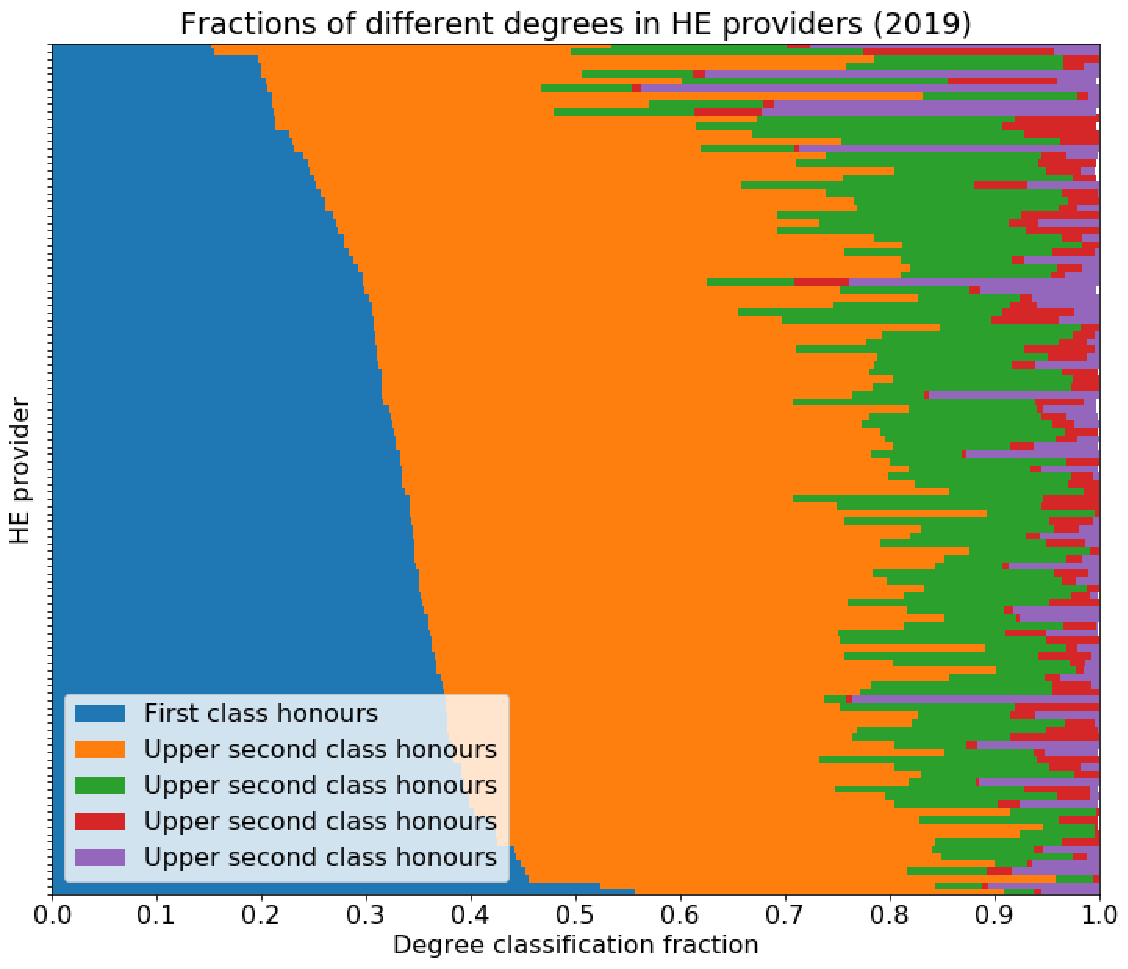
\includegraphics[width=15.24cm]{report/Q11FFF.pdf}
    \caption{The fraction of degree classification in 115 HE providers with over 1000 graduating students in academic year 2019/20. The Y axis ranks the fraction of first class honours from lowest to highest}
    \label{fig:Q11F}
\end{figure}


\section{Introduction}
% Suggested 400 words

\paragraph{Context and motivation}
\paragraph{}

Thanks to the increasing attention on education and continuous recording over decades, there are abundance data available for research on higher education. Investigation into grading has always been an active field over the world since it could help to identify latent problems and to plot a path for future generations. Rojstaczer et al \cite{Rojstaczer1}, \cite{Rojstaczer2}  tracked the evolution of American university grading over a span of 70 years, Schombert \cite{Schombert1}, \cite{Schombert2} modeled college GPA (Grade Point Average) to predict future score, and Dearden et al \cite{Dearden2011impact} pointed out that students in UK higher education system have massively increased. With more students, increase in data quantity, and better prediction models, research into university grading would become increasingly popular and valued in the future. 

However, apart from the thriving surface of college student expansion, some concerns gradually arise in recent years. According to the data \cite{HESA} from UK Higher Education Statistics Agency (HESA), the number of students obtaining a first-class honours has increased from 28\% in 2018/19 to 35\% in 2019/20. Meanwhile, multiple media \cite{news1}, \cite{news2},\cite{news3} have reported a phenomenon called "grade inflation": the increase in grade over time without a corresponding increase in students' capability. New Statesman \cite{news1} reported that the percentage of first-class students has tripled within just 20 years. The situations "a significant proportion of the year-on-year increases could still not be explained" and "an unexplained increase in firsts at almost three-quarters of universities in England" are described by BBC \cite{news2}, signifying the severity of grade inflation and how widespread it is. Meanwhile, some possible explanations are proposed by those reports, including improved student capability, more investment in academic support, the shift to outcomes-based assessment approach, and competition within top universities that reaches a prisoner's dilemma. 

\paragraph{Previous work}
\paragraph{}

From Trow et al \cite{Trow1973} defined the quality of education in 1973 to a comprehensive analysis by Bayesian multilevel modeling in 2020 \cite{BayMain}, the concern of grade inflation has continuously attracted researchers in decades. When we look closely at UK higher education data, a lot of work have been done: Richmond \cite{FancyPink} plotted the growth of first class in UK, Gershenson \cite{FancyGreen} categorized HE providers into more and less affluent schools and analyzed the difficulty to obtain a first within them, and Lackey et al \cite{USTrend} showed a similar trend in American universities. Furthermore, some explanations are being carried out: Jephcote et al \cite{BayMain} argue that most proportion of grade increase could be explained by geographical conditions \& college entry score, and Rojstaczer et al \cite{GI} categorized the growth in America into different timeline such as the Vietnam Era. 

\paragraph{Objectives}
\paragraph{}

In this work, we are focusing on exploring degree classifications between different HE providers since previous works \cite{HESA}, \cite{FancyPink}, \cite{FancyGreen} primarily focus on UK education as a whole. Because data from most recent years are not yet explored, we are investigating the variation of degree in the past six years. Differences between types of institutions from multiple perspectives are being explored by us and conclusions from \cite{BayMain}, \cite{NORDIN2019101936}, discussing the relation of multiple variables with grade, are also being examined here. 

\section{Data}
% Suggested 300 words

\begin{figure}[t]
    \centering
    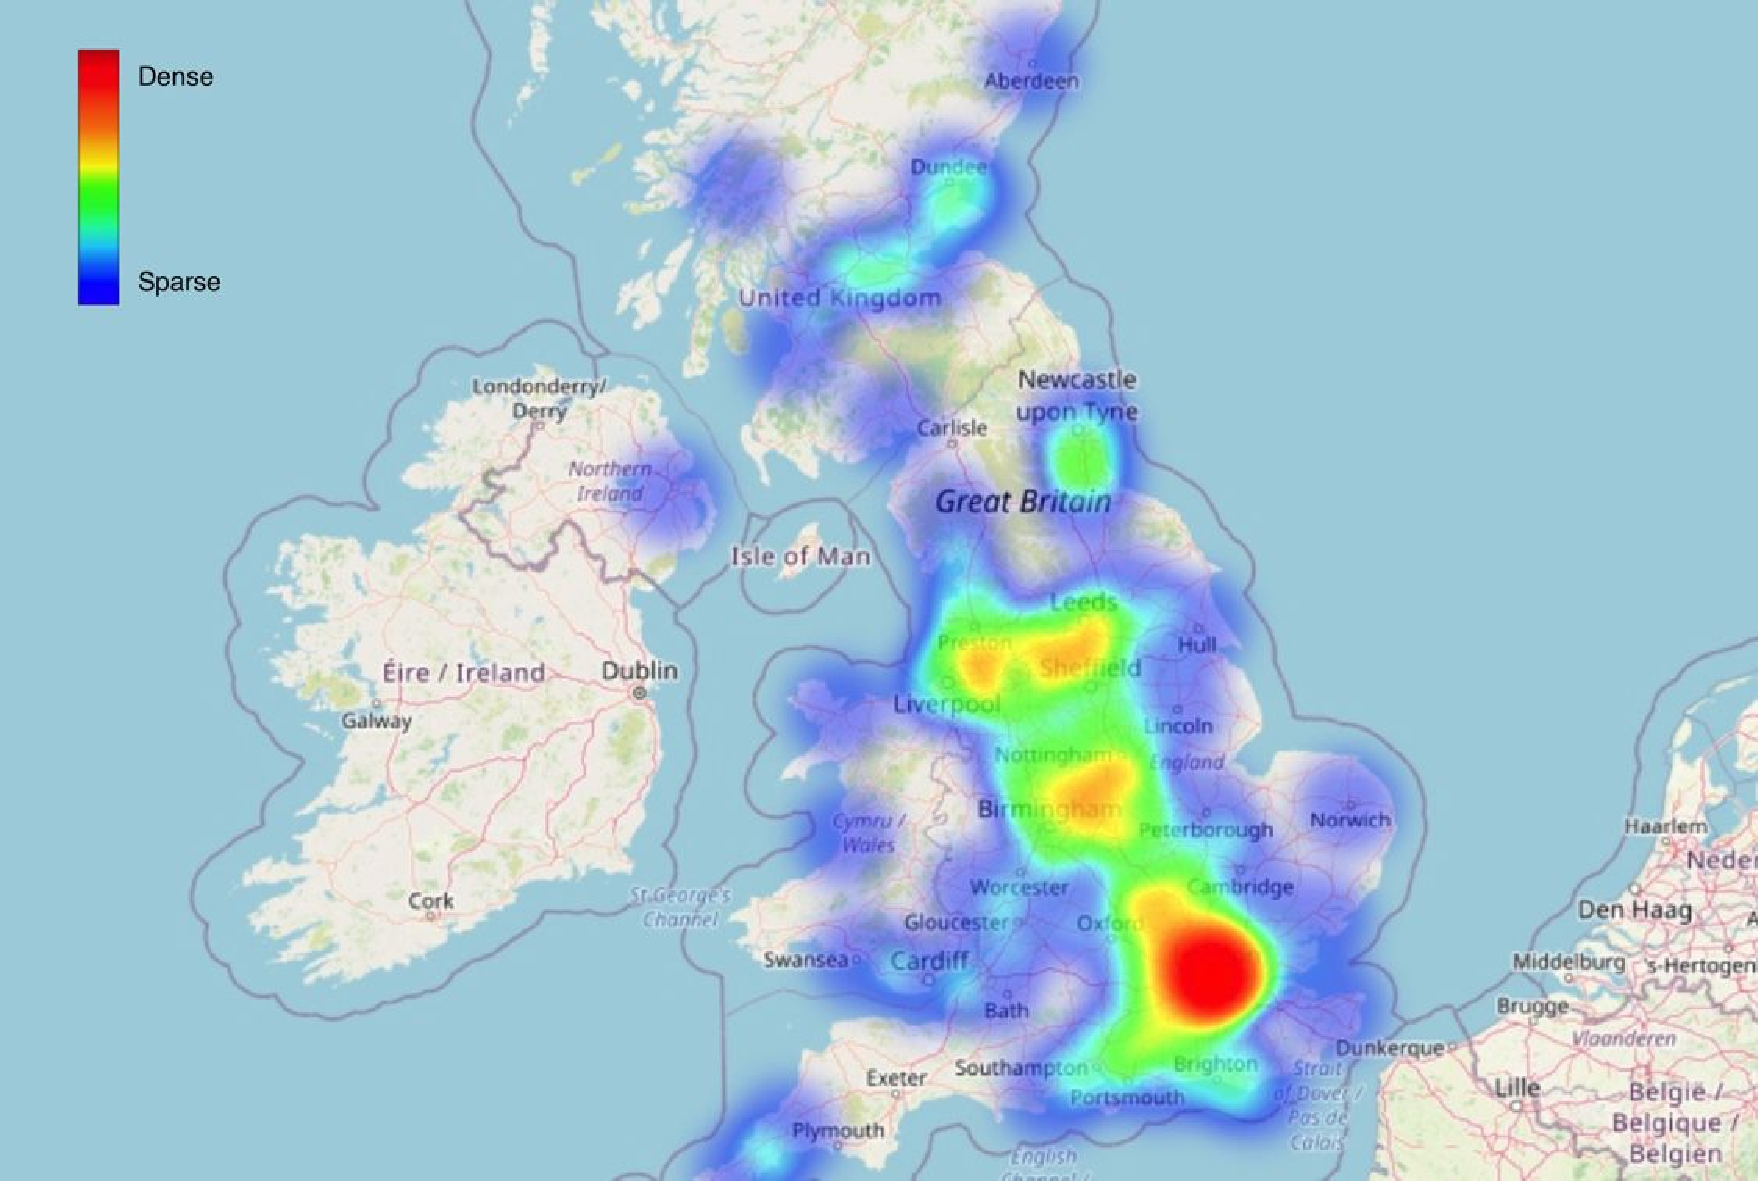
\includegraphics[scale=0.5]{report/Q22FF.pdf}
    \caption{Map showing locations of higher education providers with different fraction of first class honours in UK. More red represents the location where this fraction is high and blue represents the fraction is low. The map data is supported by OpenStreetMap, under ODbL}
    \label{fig:Q12}
\end{figure}

\paragraph{Data provenance} 
\paragraph{}

The UK higher education data, developed by relevant government and educational departments, is downloaded from the website of Higher Education Statistics Agency \cite{HESA}, the official data collection agency of UK higher education. Detailed information of each HE provider, such as their entry score and research quality, are downloaded from Complete University Guide \cite{CUG}. This dataset is created by an educational guidance company named IDP Connect \cite{IDP}. Both are publicly available datasets they are free to copy and use for any purpose according to their terms \& conditions. We have ensured that private information, such as an individual's entry score, does not appear in the datasets and would be securely disposed of after our research. 

\paragraph{Data description} 
\paragraph{}

Since there is an abundance of tables and variables, we will only picture the ones that are not self-explanatory. In the tables named by academic years, the variable UKPRN identifies each HE provider and a total of 270 institutions are being recorded. The variable FIRST DEGREE represents the number of students achieving an undergraduate degree. In subject-all.csv, the variable SUBJECT AREA is the number of students that achieved any qualification in one subject, whereas it represents that achieved an undergraduate degree (first degree) in the file subject-first.csv. The file ranking.txt contains the UK university rankings ordered from highest to lowest and other txt files list the institutes in such order. 

\paragraph{Data processing} 
\paragraph{}

We first clean all the tables by dropping any rows with NAN values and format the dataset for use. During the analysis, we only consider HE providers with more than 1000 students to remove outliers, thus 115 of 270 schools remains. To obtain the fractions of first-class and other degree classifications, we replicate the original data frame and carry out the computation of fractions. The datasets also contain some missing values: one HE provider that exist in the 2019-2020 Dataset is missing in the LOCATION dataset. To resolve this issue we manually look up this information online, and its geographical value is then added to the LOCATION dataset. To ensure the coefficients in the regression model are in proportion with one another, we normalize the data to a zero to one scale for the regression task only. 

\section{Exploration and  analysis}
% Suggested 500 words for individual report; proportionately longer
% for group projects).

\begin{figure}[t]
    \centering
    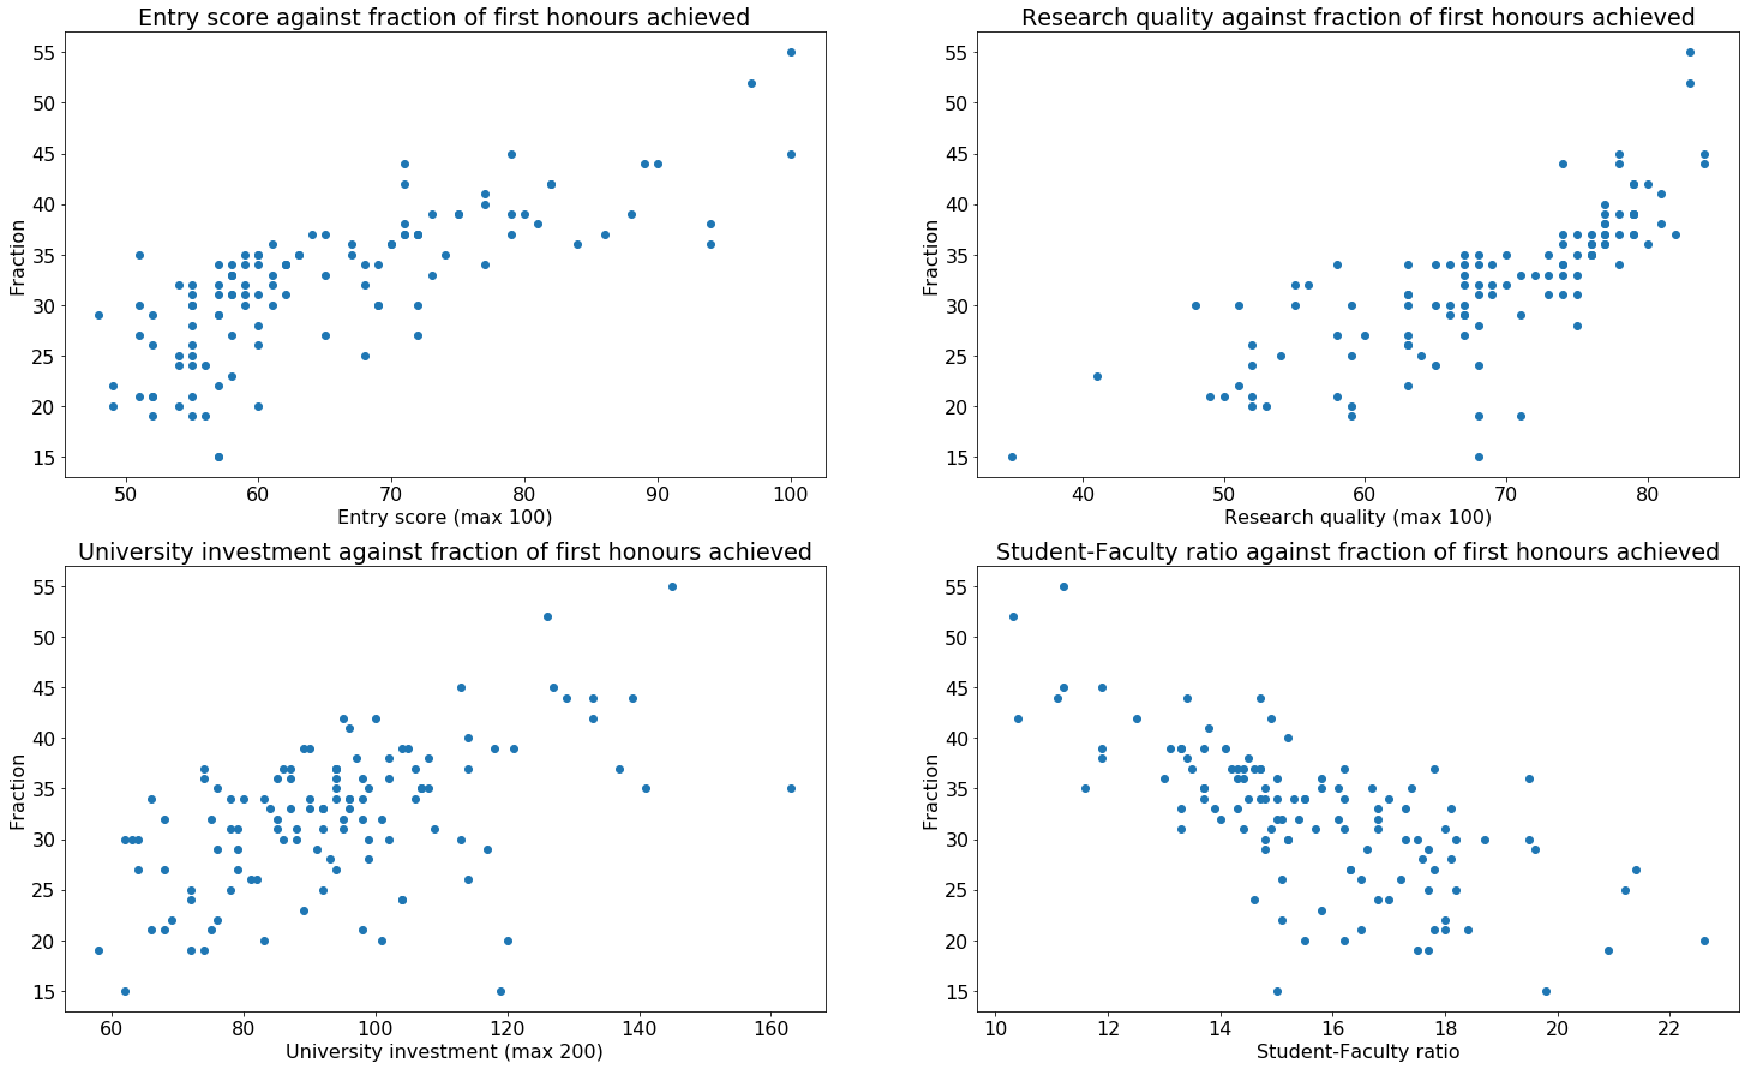
\includegraphics[width=15.24cm]{report/Q13FFF.pdf}
    \caption{Relationship of percentage of firsct class versus the four variables: Entry score, research quality, university investment and student-faculty ratio. Entry score and research quality are measured in a 0 to 100 scale. Since university investment include academic investment and facilities investment, the two are added up and it is measured in a 0 to 200 scale. }
    \label{fig:Q13}
\end{figure}



\paragraph{Distribution of degree classifications achieved in different providers}  
\paragraph{}

Although some schools such as St Mary's University College have an astonishing 100\% of first class honours, it is not sensible to compare it with large HE providers given that only 220 students graduate from this college in a year. Thus we only consider institutions with over 1000 graduates in the academic year 2019-20. In figure \ref{fig:Q11F}, we demonstrate the fraction of degree classification in HE providers by ranking it from lowest to highest percentage of first class honours. 



From figure \ref{fig:Q11F}, we could observe that there is considerable variation in degree distribution across HE providers: even when excluding outsiders (the leftmost and rightmost two institutes), the percentage of first class rises from 20\% to over 40\%. Moreover, in institutions with some of the highest fraction of firsts, lower second class, and third class almost disappeared: nearly all students achieve a high score. However, upper second class is the most common degree in most schools in the year 2019/20 and it is more common than first class by an average of 10\%. This suggests that the proportion of firsts might not be as high as that described in media \cite{news1}, \cite{news2}, although this phenomenon is worth noting in some schools. 

\begin{figure}[h]
    \centering
    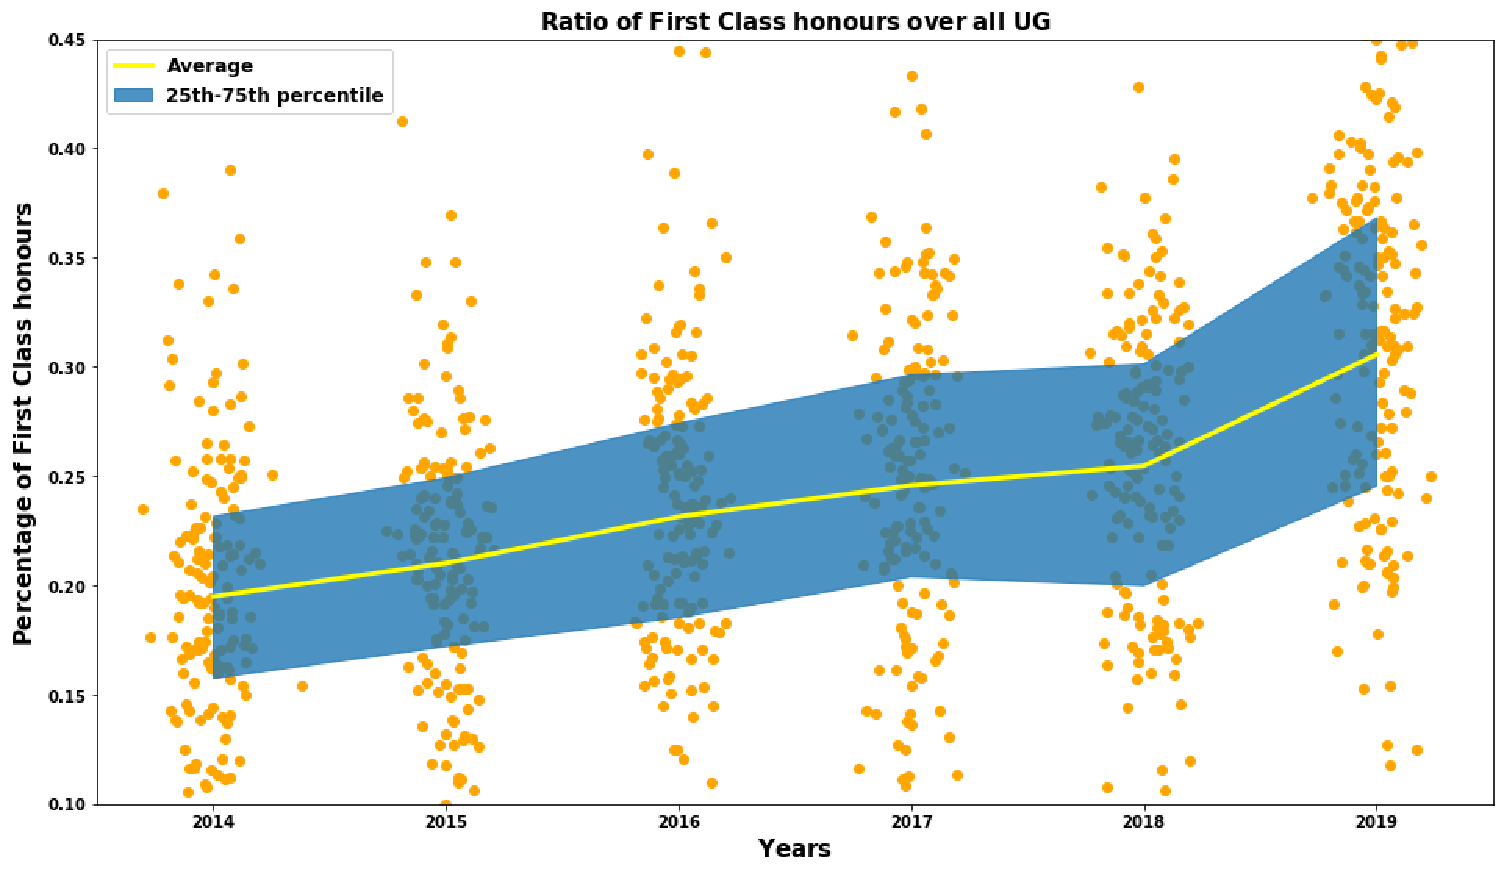
\includegraphics[width=15.24cm]{report/Q21FFF.pdf}
    \caption{The percentage of first class in all HE providers overtime. The yellow dots represent institutions in a year with some horizontal randomness to reduce overlap. The trends of average value and interquartile range are presented. }
    \label{fig:Q21}
\end{figure}


To specifically observe each HE provider, Table 1 shows the schools with highest and lowest fractions of first class and other degrees in year 2019/20. LSE ranked first in providing the most firsts and University of Stirling ranked last. 

\begin{table}[h!]
  \caption{Institutions providing the highest to lowest fraction of different degree classifications in academic year 2019-20. The top and bottom three HE providers of each degree classification are shown. }
  \label{tab:example1}
\begin{tabular}{lrrrrrrr}
\hline
\textbf{}&\textbf{First Class Honours}&\textbf{Upper Second Class-}&\textbf{Lower Second Class-}\\
               &                            &\textbf{Honours}            &\textbf{Honours}      \\
\hline
\textbf{1}&\text{London School of Economics}&\text{University of Chichester}&\text{BIMM Limited}&\tabularnewline
\textbf{2}&\text{Imperial College London}&\text{University of Winchester}&\text{The Open University}&\tabularnewline
\textbf{3}&\text{University College London}&\text{Bath Spa University}&\text{University of Bedfordshire}&\tabularnewline
\dots&\dots&\dots&\dots\tabularnewline
\textbf{113}&\text{University of Winchester}&\text{University of Dundee}&\text{The University of Oxford}&\tabularnewline
\textbf{114}&\text{Open University}&\text{Robert Gordon University}&\text{University College London}&\tabularnewline
\textbf{115}&\text{University of Stirling}&\text{University of West Scotland&\text{University of Cambridge}&\tabularnewline
\hline
\end{tabular}
\end{table}

We also explored the locations of HE providers with different fraction first class honours within the UK. Figure \ref{fig:Q12} maps the institutions with different percentage of firsts. Schools with a higher rate of first class accumulate in London, while schools in Scotland, Wales \& Northern Ireland have a lower fraction of firsts. This finding corresponds with Table 1: the top three universities providing highest fraction of first class all located in London. Following the result of Rojstaczer et al \cite{Rojstaczer1}, we infer that the scale effect of those regions -- most abundant resources and elite instructors tends to cluster in those areas -- might be the reason for the accumulation of institutes providing high score. 




To look into the reason that the degree distribution might be the case, we ask ourselves the following question inspired by the result of \cite{BayMain}: is there a relationship between the percentage of first class honours and those variables? 

\begin{itemize}
    \item Universities and College Admissions Service (UCAS) entry scores, 
    \item Research quality, 
    \item University investment 
    \item Student-faculty ratio
\end{itemize}

Figure \ref{fig:Q13} is answering this question by plotting the relationship of fraction of first class versus those four variables. We could observe that the student's ability when entering each HE provider, measured by the average UCAS entry scores of each institution, is directly proportional to the fraction of first class achieved by students in the institute. Similar relation could be viewed from the relationship of the college's research quality and fraction of firsts. Although the relation between university investment and grade is still directly proportional, it is not as strong as that of UCAS entry score and research quality. Moreover, the student-staff ratio is inversely proportional to the percentage of firsts. 


\begin{figure}[h]
    \centering
    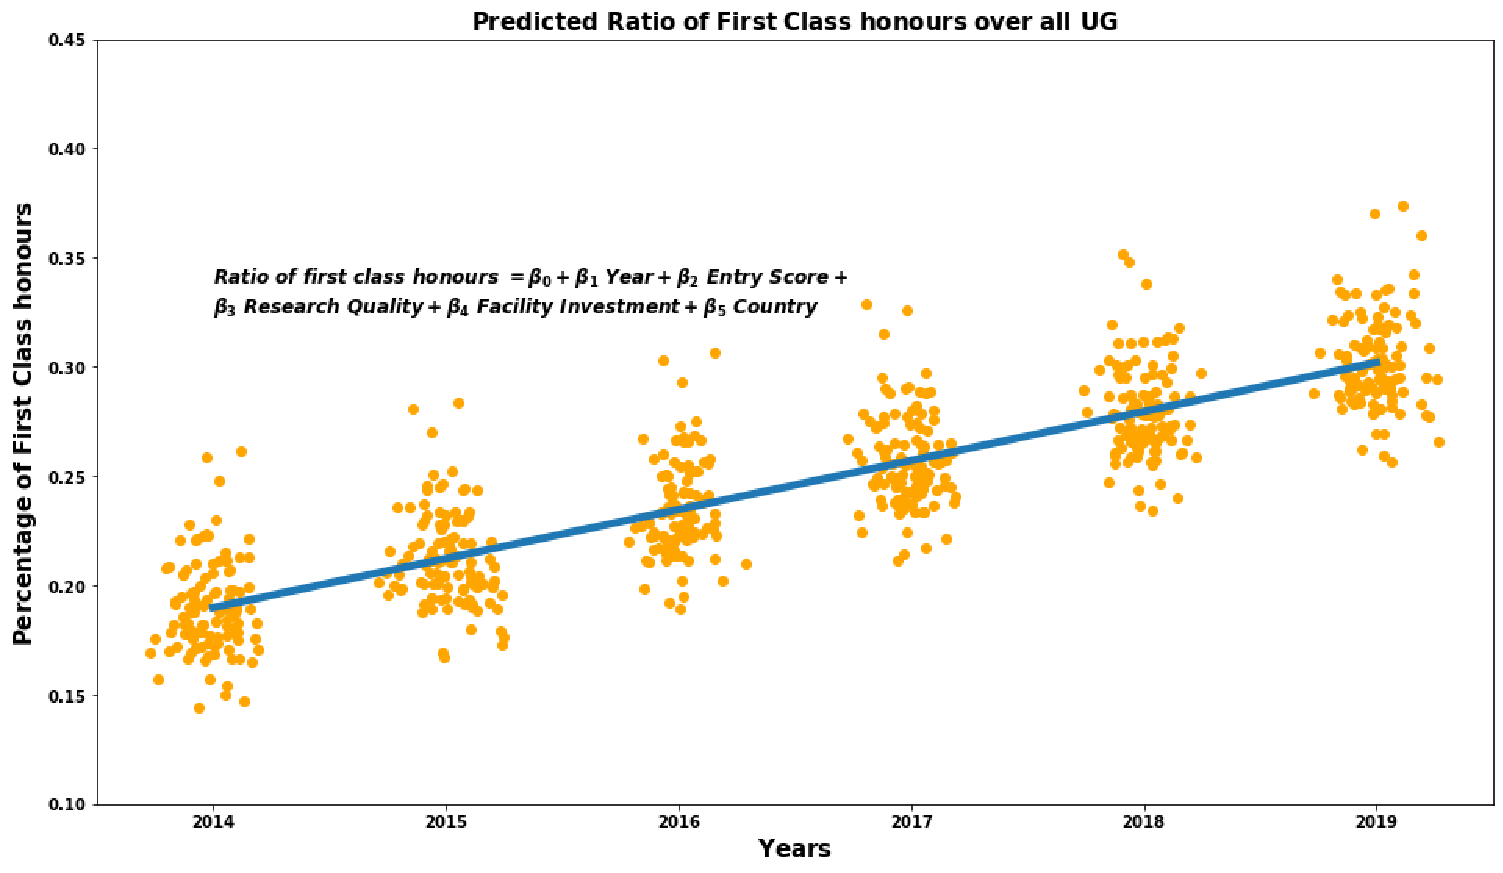
\includegraphics[width=15.24cm]{report/Q22FFF.pdf}
    \caption{Using multiple regression model to predict the percentage of first class in all HE providers overtime. The blue line is the regression line and the yellow dots represent institutions in a year with some horizontal randomness to reduce overlap. }
    \label{fig:Q22}
\end{figure}

To sum up, when observing HE providers, the ones with greater expenditure on academic performance, better research output, more instructors teaching fewer students, and more capable students in entry tend to award more first honors. Although this finding corresponds with the results in Jephcote et al \cite{BayMain}, the specific strength of each variable yet remains unknown and a cause and effect have not been found. 



\paragraph{Grades overtime }  
\paragraph{}

In Figure \ref{fig:Q21}, we investigate the percentage of firsts in all HE providers from year 2014 to 19. The region between 25\% and 75\% percentile is indicated and we could observe its year-by-year increase in the whole spectrum. This indicates that the percentage of firsts is indeed strictly increasing over time. Also, the increase from year 2018/19 to 19/20 is the greatest. 

\begin{figure}[t]
    \centering
    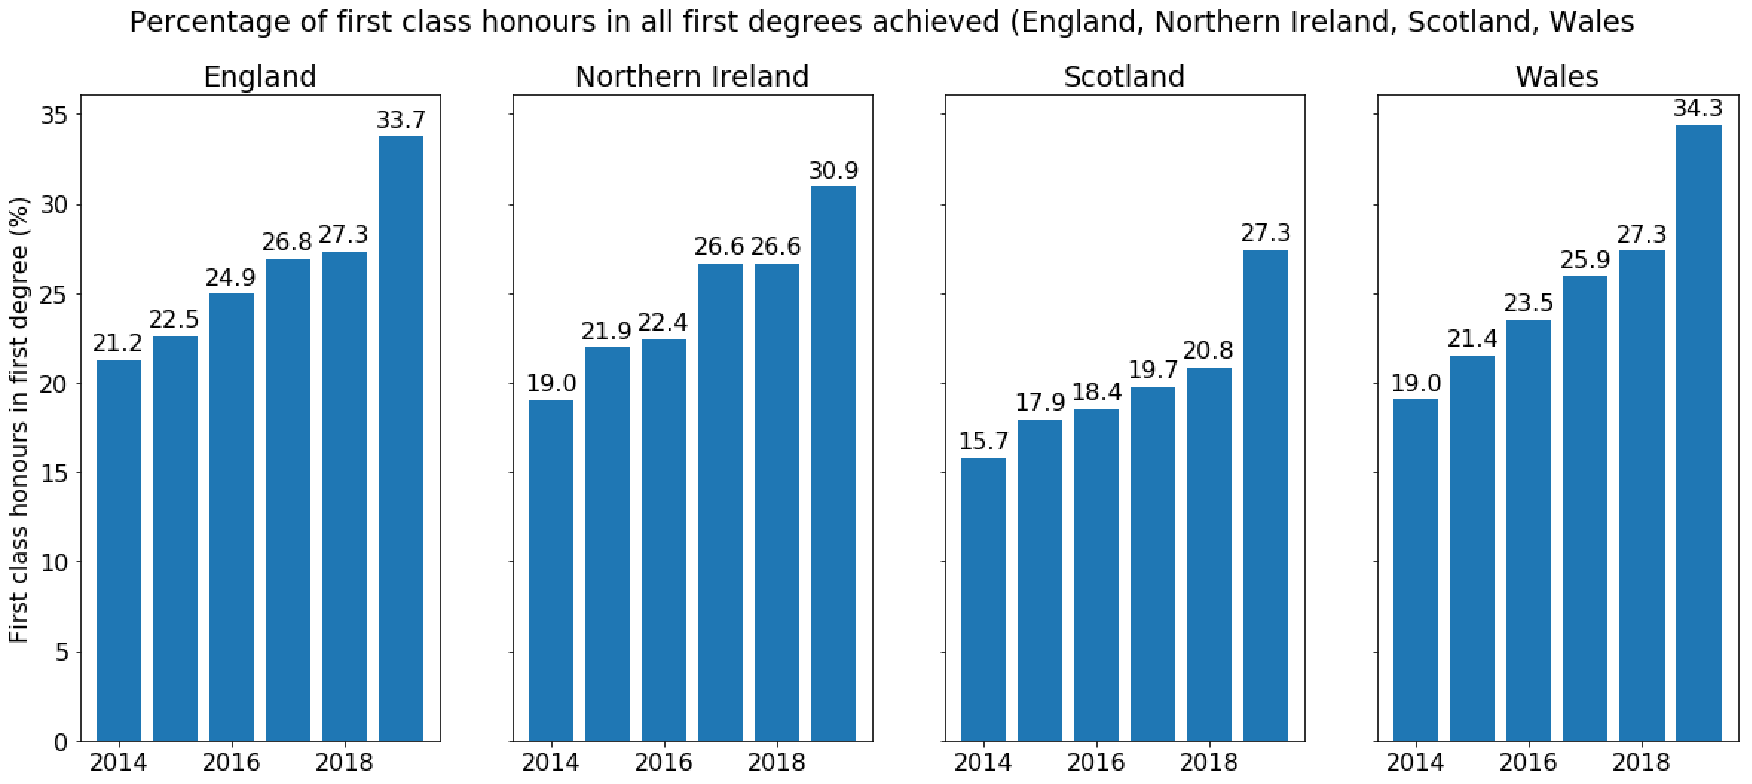
\includegraphics[width=15.24cm]{report/Q31FFF.pdf}
    \caption{First class rates for higher education institutes across four countries of the United Kingdom, from 2014/15 to 2019/20. This result is correspond to that of Richmond \cite{FancyPink}}
    \label{fig:Q31}
\end{figure}

However, an increasing percentage of firsts does not necessarily indicate the phenomenon of grade inflation. It is possible that the variation of the four variables above contributes to the increase in grade thus the phrase "inflation" would not hold. To explain the growth of grade, we model the fraction of first-class honors by the following multiple regression model in Equation1 (we only consider the three directly proportional variables here): 

\begin{equation}
    \label{eq1}
    \mathrm{Fraction.of.firsts}_{t} = \beta_{0}
    &+ \beta_{1}  \mathrm{Year}_{t} \tabularnewline
    &+ \beta_{2}  \mathrm{Entry.score}_{t}    \tabularnewline
    &+ \beta_{3}  \mathrm{Research.quality}_{t} \tabularnewline
    &+ \beta_{4}  \mathrm{Invertment}_{t} \tabularnewline
    &+ \beta_{5}  \mathrm{Country}_{t}   \tabularnewline
\end{equation}
\vspace{\baselineskip}

For the categorical variables Years and Country (of UK), we convert it to a numeric variable by encoding. The data is also normalized into a zero to one scale to fight any disparities in the variable size and ensured the parameters in the multiple regression model are in proportion with one another. 

\begin{table}[h!]
\label{table2}
\centering
  \caption{Statistical summary for the parameters of the multiple regression model examinating precentage of first class (Y variable) of UK higher education providers. }
  \label{tab:example1}
\begin{tabular}{lrrrrrrr}
\hline
\hline
\textbf{Parameters}&\textbf{coefficient}&\textbf{Standard error}&\textbf{T value}&\textbf{P value}\\
\hline
\textbf{Intercept}&$-44.3790$&$2.5639$&$-17.3090$&$0$&\tabularnewline
\textbf{Year}&$0.0221$&$0$&$10926.52$&$0$&\tabularnewline
\textbf{Entry score}&$0.0012$&$0.00018$&$6.8950$&$0$&\tabularnewline
\textbf{Research Quality}&$0.0006$&$0.00017$&$3.6301$&$0.0003$&\tabularnewline
\textbf{Facility Invest}&$0.0004$&$0.00017$&$2.5082$&$0.0124$&\tabularnewline
\textbf{Country in UK}&$-0.0117$&$0.00272$&$-4.3025$&$0.00002$&\tabularnewline
\hline
\hline
\textbf{R-squared:          0.413}&\tabularnewline
\textbf{Adj. R-squared:     0.408}&\tabularnewline
\textbf{95\% confidence interval:     [0.211,0.295]}&\tabularnewline
\hline
\end{tabular}
\end{table}


Outputs from the multiple regression are shown in Table 2 and the regression line is shown in Figure \ref{fig:Q22}. Difference in country of UK has the highest absolute value of coefficient, thus geographical condition contributes the most to difference in the percentage of first-class honors. Measured by the institute's UCAS entry score, student's ability when entering higher education is the second highest factor. An increase of 1 in the normalized entry score predicts an increase of 0.0012 in the normalized percentage of firsts. The influence of research quality and investment comes after. 


P values are also calculated for each parameter and they are all < 0.05. This means that all variables are likely to be meaningful predictors for grade. The 95\% confidence interval is [0.211, 0.295], indicating 95\% of first-class honors is between those two numbers. Furthermore, the addressed coefficient of determination $R^2$ is 0.41, suggesting nearly 60\% of the variance in grade could not be explained by our predictors. Thus the phenomenon of grade inflation may exist since our result matches the media report claiming "half of the results could not be explained"\cite{news3}. The result from our multiple regression model is consistent with that of Bayesian multilevel modeling from Jephcote et al \cite{BayMain}, thus their conclusion is confirmed. 







\paragraph{Differences between institutions}  
\paragraph{}

\begin{figure}[t]
    \centering
    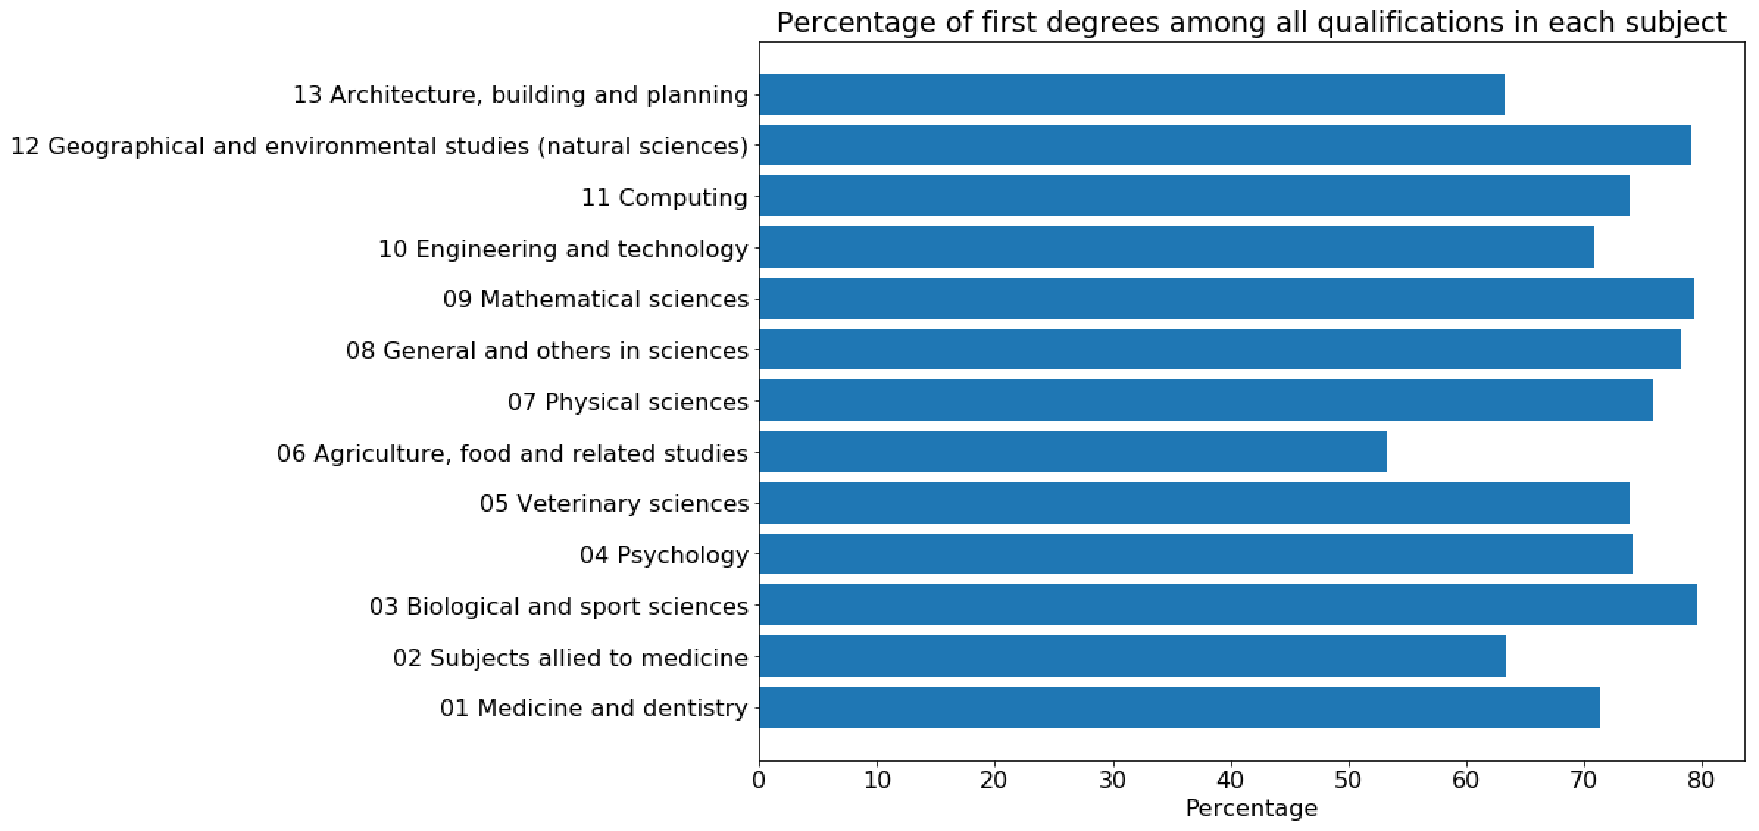
\includegraphics[width=15.24cm]{report/Q32FFF.pdf}
    \caption{Proportions of first degree achieved in each subject area.}
    \label{fig:Q32}
\end{figure}




Figure \ref{fig:Q31} summarizes the percentage of first class in higher education institutes, across the four nations of UK, from academic year 2014/15 to 2019/20. Although Figure \ref{fig:Q12} shows the fraction of firsts is significantly higher in England in year 2019/20, the year-on-year increase in all four nations is roughly comparable and all experience a sharp growth in the year 2019/20. This growth pattern corresponds with Figure \ref{fig:Q21} and we presume that the sudden increase might be caused by the impact of Covid-19. The proportion of firsts in England, Scotland and Northern Ireland has risen about 12\% over the five-year period, while Wales have risen the most, for 15.3\%. 



To state the differences between subjects studied, we present Figure \ref{fig:Q32}. It demonstrates a considerable variation in the percentage of firsts awarded across different subjects. Biological and sport science awards the highest proportion of Firsts at nearly 80\%, while Agriculture, food and related studies award just 53\% of degrees as firsts. In general, science subjects that require more resoning skills and less field practice award higher ratio of firsts and subjects strongly depend on hands on experience, agriculture and medicine, provide lower fraction of first degree. We argue that this difference might contribute to the variation between subjects. 


To investigate the differences between the size of institutions, we apply the multiple regression formulae to observe how much schools with different numbers of students deviate from the predicted grading. The result is shown in figure \ref{fig:Q33} that categorizes all schools into three orders of magnitude: less than 1000 graduates, between 1000 \& 5000 and above 5000. The distribution of the largest institutions is roughly normal with little incline to the higher end. Schools with graduates between 1000 \& 5000 are normal with minimal derivation from predicted value, suggesting they are the best representation of all schools. What is perhaps most striking is their smallest institutions: their distribution is about 5\% lower than other HE providers and considerably positively skewed. Moreover, if we set the yellow curve as reference, nearly half of the smallest schools are below its 95\% confidence interval. This is why we did not consider schools below 1000 graduates in the first place: to eliminate outliers. Having a glance at the raw data, we notice that a considerable amount of schools have zero first-class honors and single-digit total graduates. Generally speaking, the larger the size of the HE provider, the more normal its distribution is. 


\begin{figure}[h]
    \centering
    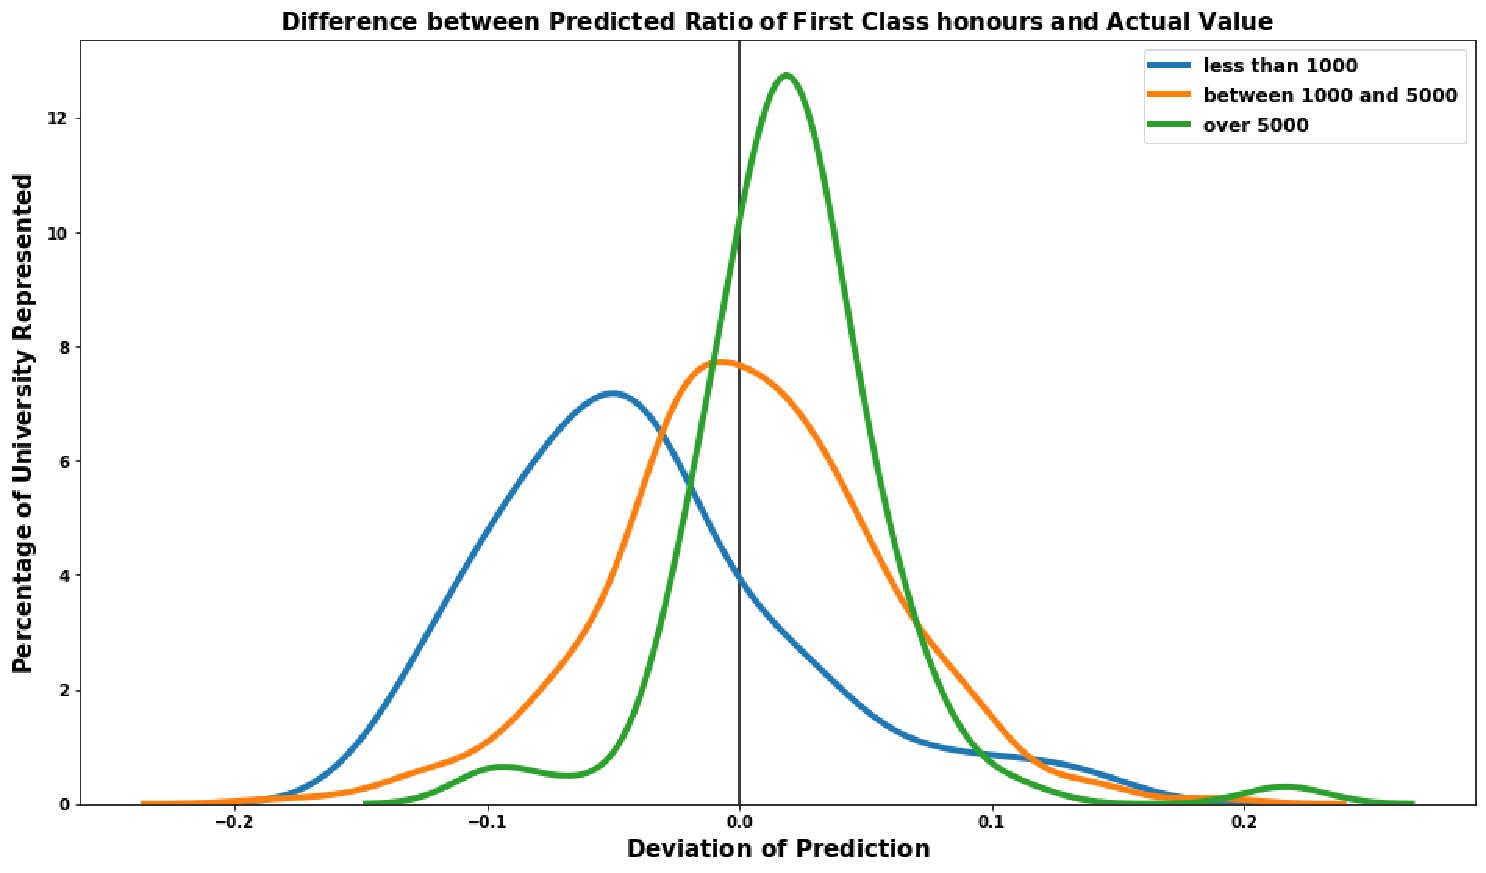
\includegraphics[width=15.24cm]{report/Q33FFF.pdf}
    \caption{Histogram of differences between the ratio of first class predicted by the multiple regression model and that of the institutions with different size: less than 1000 graduates, between 1000 and 5000, above 5000 graduates. }
    \label{fig:Q33}
\end{figure}



\section{Discussion and conclusions}
% Suggested 400 words.

\paragraph{Summary of findings and related works} 
\paragraph{}

In this work, we first discovered a considerable grade variation across HE providers: at most twice in first-class honors. But the most common class and comparison with grade distribution in US \cite{USTrend} suggest that the proportion of first-class honors in UK might not be as high as that described in media. We then point out that the universities providing the highest fraction of firsts would locate in London by tables and map. Directly proportional relationships of first-class honors with entry score, investment and research quality are found. Also, the lower the student-staff ratio, the higher the grade is. Furthermore, we confirmed that the percentage of firsts is indeed increasing from 2014 to 2019 and recognized that nearly 60\% of grade increase could not be explained. This is achieved by adopting a multiple regression model that also confirmed the order of variable influence concluded by Jephcote et al \cite{BayMain}: locational impact is the greatest, followed by influence of entry score, research quality and investment. Finally, we state that the annual grade increase in all four nations are roughly the same, visualize a variation in the percentage of firsts across different subjects. We also explain the reason to view smaller HE providers as outliers and conclude that the larger the institution is, the better we could predict its rate of first class by regression. 

\paragraph{Comparison with other works}
\paragraph{}

Further research suggests that the phenomenon of grade inflation is a global phenomenon: United States \cite{Rojstaczer2}, Sweden \cite{WIKSTROM2005309}, Israel \cite{doi} and many other countries all experience the same increase in top grade. Researches on greater length of time \cite{BayMain} \cite{Rojstaczer2} also indicate that higher education grade has been increased for decades and mapping its growth trend by historical periods is possible \cite{doi10}. Data from Google Trend \cite{GT} expresses a similar story: the search frequency for the word "grade inflation" remains relatively constant in the past ten years and the word is interested by people all around the world. 


\paragraph{Strengths, limitations and improvements} 
\paragraph{}

Although causality could not be found, we are still proud of our exploration of variables that are related to grade increase. Not only we answered the question "why the grade increase might be the case?", but we also applied multiple regression to predict the trend of grade growth. By searching related variables, we connected three separate questions together in a rough trail - prediction - evaluation manner and provided explanation for the public concerning problem of "grade inflation". 

Limitations are also present in our work and require improvement by future works. Instead of data from the year 2013/14 to 19/20, longer time spends — ten years or even decades — could be put into consideration. When discussing grade patterns over time, we did not consider variation in each HE provider. In future works, we would explore the institutions with the highest and lowest increase in the proportion of firsts. Corresponding to its distribution pattern, Figure \ref{fig:Q11F} could also be explored through time to investigate the movement of each HE provider along the Y-axis. Furthermore, although experiment that aims to explore the cause and effect of entry score, research quality and investment on grade would almost be impossible, Granger Causality Test could be applied in the future to provide insights to improve the quality of higher education. 

\bibliographystyle{unsrt}
\bibliography{fds-project}
\end{document}
